\documentclass[12pt,a4paper]{article}
\usepackage[T1]{fontenc}
\usepackage[utf8]{inputenc}
\usepackage{mathptmx,courier}
\usepackage[a4paper,left=2.3cm,right=2.0cm,top=3.3cm,bottom=2.8cm,headheight=34pt,headsep=0.75cm,footskip=0.9cm]{geometry}
\usepackage{graphicx,xcolor,array,tabularx,longtable,enumitem,setspace}
\usepackage{tikz,eso-pic,fancyhdr,amsmath,amssymb,float,listings,url}
\usetikzlibrary{positioning}
\usepackage[labelfont=bf,labelsep=colon,skip=6pt]{caption}
\usepackage[hidelinks]{hyperref}
\setlength{\parindent}{0pt}\setlength{\emergencystretch}{3em}\renewcommand{\arraystretch}{1.25}\setstretch{1.12}\setlength{\parskip}{5pt}
\definecolor{rvred}{RGB}{105,22,30}\definecolor{rvblue}{RGB}{35,65,100}
\newcommand{\ProjectTitle}{Explainability of a Frozen AI Text Detector}
\newcommand{\AcademicYear}{2026--2027}
\newcommand{\chap}[2]{\clearpage\phantomsection\label{#1}\addcontentsline{toc}{section}{#2}\begin{center}{\bfseries\fontsize{16}{20}\selectfont #2}\end{center}\vspace{0.2cm}}
\newcommand{\sect}[1]{\par\vspace{3pt}\phantomsection\addcontentsline{toc}{subsection}{#1}{\bfseries\fontsize{14}{17}\selectfont #1}\par\vspace{2pt}}
\newcommand{\subsect}[1]{\par\vspace{2pt}{\bfseries\fontsize{12}{15}\selectfont #1}\par}
\AddToShipoutPictureBG{\begin{tikzpicture}[remember picture,overlay]\draw[line width=1.5pt]([shift={(2.0cm,2.6cm)}]current page.south west) rectangle ([shift={(-1.8cm,-3.05cm)}]current page.north east);\end{tikzpicture}}
\fancypagestyle{main}{\fancyhf{}\fancyhead[L]{\parbox[b]{0.78\textwidth}{\fontsize{9}{11}\selectfont \ProjectTitle}}\fancyhead[R]{\fontsize{9}{11}\selectfont \AcademicYear}\fancyfoot[L]{Department of AIML, RVCE}\fancyfoot[R]{\thepage}\renewcommand{\headrulewidth}{0pt}\renewcommand{\footrulewidth}{0pt}}
\pagestyle{main}
\begin{document}
\newgeometry{top=3.4cm,bottom=2.9cm,left=2.5cm,right=2.3cm}\thispagestyle{empty}
\begin{center}

\includegraphics[height=2.1cm]{images/rvce_logo.png}\hfill\raisebox{1.1cm}{
\includegraphics[height=1.0cm]{images/tagline.png}}\\[0.6cm]
{\bfseries\fontsize{16}{22}\selectfont\color{rvred} DEPARTMENT OF\\[5pt] ARTIFICIAL INTELLIGENCE AND MACHINE LEARNING}\\[0.5cm]

\includegraphics[width=2.2cm]{images/emblem_small.png}\\[0.7cm]
{\bfseries\fontsize{19}{27}\selectfont \ProjectTitle}\\[0.7cm]
{\bfseries\fontsize{14}{19}\selectfont PROJECT REPORT}\\[0.4cm]
{\bfseries\fontsize{13}{18}\selectfont Submitted by}\\[0.3cm]
{\bfseries\fontsize{13}{18}\selectfont Student name: Not provided\\USN: Not provided}\\[0.55cm]
{\bfseries\fontsize{12}{17}\selectfont Course: Not provided \quad Semester: Not provided}\\[0.5cm]
{\bfseries\fontsize{12}{17}\selectfont Under the Guidance of\\Guide name and designation: Not provided}\\[0.8cm]
{\bfseries\fontsize{13}{18}\selectfont RV College of Engineering\\Bengaluru--560059}\\[0.3cm]
{\bfseries\fontsize{13}{18}\selectfont Academic Year \\ \AcademicYear}
\end{center}\restoregeometry\newpage
\newgeometry{top=3.4cm,bottom=2.9cm,left=2.5cm,right=2.3cm}\thispagestyle{empty}
\begin{center}{\bfseries\fontsize{17}{22}\selectfont\color{rvred} RV COLLEGE OF ENGINEERING\textsuperscript{\textregistered}}\\[5pt]
{\small (Autonomous Institution Affiliated to Visvesvaraya Technological University, Belagavi)}\\[0.5cm]
{\bfseries\fontsize{15}{20}\selectfont DEPARTMENT OF\\ARTIFICIAL INTELLIGENCE AND MACHINE LEARNING}\\[0.5cm]

\includegraphics[width=3.3cm]{images/emblem_cert.png}\\[0.5cm]
{\bfseries\fontsize{15}{20}\selectfont\underline{REPORT INFORMATION}}
\end{center}
This document follows the title-page and report layout of the supplied RVCE project-report template. It documents a completed research and implementation project using the materials available in the project repository. Administrative details not supplied by the project owner are explicitly marked ``Not provided''; no student, course, guide, or approval information has been inferred.\\[0.6cm]
\textbf{Project:} \ProjectTitle\\
\textbf{Student name and USN:} Not provided\\
\textbf{Course and semester:} Not provided\\
\textbf{Guide:} Not provided\\
\textbf{Evidence basis:} committed source code, experiment configuration, generated metrics, figures, and report artifacts in the project repository.
\restoregeometry\newpage
\thispagestyle{plain}\begin{center}{\bfseries\fontsize{16}{20}\selectfont ABSTRACT}\end{center}
Machine-generated text detectors are often presented through a single accuracy value, although their behavior may change across domains, generators, languages, and writing styles. This project evaluates and interprets one frozen Random Forest detector trained on eight stylometric statistics. The model artifact and its source revision are pinned and checksum-verified; no detector is retrained. A balanced sample of 5,000 human and 5,000 AI examples was drawn with seed 42 from the English RAID training split. Model performance was 60.99\% accuracy and 0.6445 ROC-AUC; AI-class precision, recall, and F1 were 59.66\%, 67.90\%, and 63.51\%. InterpretML 0.6.10 was used to produce global Morris sensitivity and partial dependence summaries, and LIME and Kernel SHAP local explanations for one example in each actual/predicted outcome category. Average word length ranked highest by Morris sensitivity, but rankings and local contributions describe the sampled model behavior and are not causal evidence. A one-feature-at-a-time perturbation analysis produced 14 label flips among 96 synthetic feature changes. The experiment documents reproducible settings, errors, explanations, and limitations. Results do not establish reliable authorship attribution and should not be used to accuse individuals of AI use.

\textbf{Keywords:} interpretable machine learning, AI-generated text detection, stylometry, InterpretML, LIME, SHAP, robustness, responsible AI
\newpage\tableofcontents\newpage\listoffigures\newpage\listoftables\newpage

\chap{ch:intro}{CHAPTER 1: INTRODUCTION}
\sect{1.1 Background}
Large language models can generate fluent text, increasing interest in automated detection. A detection score, however, is conditional on the model, evaluation sample, domain, writing style, and operating threshold. A detector that performs moderately on a balanced sample may still make consequential errors, especially when class prevalence differs in use. Interpretable machine learning can help audit which inputs influence a fixed model's outputs, but an explanation is not proof that a decision is correct or that a text has a particular author.

\sect{1.2 Project description}
This project studies the frozen \texttt{dinisds/stylometric-ai-detector} model, a scikit-learn RandomForestClassifier using eight hand-crafted text statistics. The implementation evaluates the published artifact against a sampled RAID dataset and uses InterpretML-compatible methods to describe global and local model behavior. The project does not train a detector, alter the published decision threshold, or claim that a detector can establish authorship.

\sect{1.3 Problem statement}
A user of a black-box or externally trained AI-text detector needs to understand both its measured performance on a declared sample and the feature patterns behind its outputs. The problem is to create a reproducible evaluation and interpretation workflow for a pinned frozen detector, while reporting errors, feature definitions, explanation assumptions, and limitations in a way that prevents attribution claims beyond the evidence.

\sect{1.4 Objectives and scope}
Objectives were to: (i) pin and safely load the published estimator; (ii) sample a balanced independent-source evaluation set; (iii) compute conventional classification metrics; (iv) generate global sensitivity and partial dependence analyses; (v) explain four representative outcome cases with LIME and Kernel SHAP; (vi) explore bounded one-feature changes; and (vii) preserve the implementation and results in a Git repository. Scope is restricted to one English, pooled sample and one model artifact. It does not include retraining, threshold selection, multilingual evaluation, causal inference, or user-level authorship judgments.

\sect{1.5 Organization}
Chapter 2 reviews 25 papers. Chapters 3--5 describe objectives, methodology, and implementation. Chapter 6 reports results and limitations; Chapter 7 concludes; Chapter 8 lists future work.

\chap{ch:lit}{CHAPTER 2: LITERATURE SURVEY}
\sect{2.1 Detection signals and benchmark design}
Gehrmann et al. (2019) introduced GLTR, visualizing token likelihood patterns to help people inspect generated text. Uchendu et al. (2021) established TURINGBENCH with 200,000 examples and 20 model labels, showing the value of explicit shared tasks. Rodriguez et al. (2022) studied cross-domain GPT-2 technical-text detection and showed that domain adaptation matters. Liang et al. (2023) found that several detectors disproportionately flagged non-native English essays, warning that regularity can proxy for language background. Mitchell et al. (2023) proposed DetectGPT using probability curvature on perturbed text; its scoring access and compute needs differ from a frozen feature-based classifier. Yang et al. (2024) proposed DNA-GPT, comparing n-gram divergence against regenerated continuations, which depends on query access to a relevant generator.

\sect{2.2 Generalization, attacks, and practical evaluation}
Macko et al. (2023) broadened evaluation to 11 languages in MULTITuDE. Wang et al. (2024) introduced M4 to evaluate multiple generators, domains, and languages, documenting generalization challenges. Li et al. (2024) evaluated 27 generators in the MAGE in-the-wild benchmark and found difficult out-of-distribution settings. Bao et al. (2024) made probability-curvature detection more efficient with Fast-DetectGPT while retaining language-model access assumptions. Verma et al. (2024) introduced Ghostbuster, a trained feature-based detector using weaker models, tested across writing domains. Hans et al. (2024) proposed Binoculars, contrasting related language-model behavior in a zero-shot score. Dugan et al. (2024) released RAID, with over six million examples and multiple domains, attacks, generators, and decoding settings; the present work samples only a small balanced subset. Wang et al. (2024) stress-tested detectors under editing, paraphrasing, co-generation, and prompt attacks, finding substantial vulnerability. Sadasivan et al. (2025) analyzed paraphrase attacks and the fundamental difficulty of reliable detection under small changes. Tufts et al. (2025) showed practical importance of true-positive rates at fixed false-positive rates. Doughman et al. (2025) examined style and readability transformations that can alter detector performance.

\sect{2.3 Surface features and linguistic explanation}
Dutta Chowdhury et al. (2026) studied formatting and surface-feature confounds, illustrating a Clever Hans risk when dataset conventions become shortcuts. El Attar et al. (2026) analyzed 284 linguistic features across 30 models and ten domains, finding that some signals are more stable than others. Xia et al. (2026) related generalization shifts to linguistic characteristics across prompts, models, and datasets. Together, these papers caution that interpretable style cues can be predictive within one dataset without being stable indicators of authorship.

\sect{2.4 Explanation methods}
Ribeiro et al. (2016) proposed LIME, a local surrogate whose result depends on the perturbation neighborhood. Lundberg and Lee (2017) unified additive feature attribution methods through SHAP; Kernel SHAP approximates contributions relative to a background distribution. Morris (1991) developed elementary effects for screening influential inputs, not estimating causal effects. Friedman (2001) established partial dependence as an average model response over observed values, with cautions when features are correlated or combinations implausible. Nori et al. (2019) introduced InterpretML as a common framework for glassbox and black-box interpretability methods. These methods give complementary views but do not resolve causal interpretation, distribution shift, or misuse.

\sect{2.5 Research gap and project position}
The literature documents distribution shift, attacks, benchmark artifacts, and fairness concerns, alongside a wide range of explanation methods. This project contributes a compact, reproducible case study: it preserves one detector unchanged, evaluates it on a pinned and balanced RAID sample, and describes its global and local feature behavior with explicit reference-sample assumptions. The central gap addressed is transparency about one deployed-style detector's behavior--not development of a universally reliable detector. Full annotations and source links for all 25 papers are in \texttt{literature\_survey.md}.

\chap{ch:objectives}{CHAPTER 3: OBJECTIVES AND DELIVERABLES}
\sect{3.1 Functional objectives}
The pipeline loads a pinned model artifact after checking SHA-256, extracts its eight expected inputs, evaluates labels and probabilities, gates the InterpretML adapter against the original probabilities, computes global explanations, generates local explanations for four outcome categories, and records what-if results. Reports preserve dataset and model provenance and expose figures and machine-readable outputs.

\sect{3.2 Non-functional objectives}
Reproducibility is supported through pinned repository revisions, fixed random seeds, recorded package versions, configuration, source code, output reports, and committed figures. Auditability is supported by feature definitions, sample IDs and provenance. Safety is supported by a controlled opt-in before loading the Joblib artifact and by warnings against authorship claims.

\sect{3.3 Delivered outcomes}
The completed repository includes reusable Python modules, an executable experiment notebook, a pinned experiment configuration, evaluation metrics, explanation outputs, figures, Markdown and HTML reports, the detailed literature survey, and this formal report. The large model and full dataset are downloaded at runtime rather than stored in Git.

\chap{ch:method}{CHAPTER 4: METHODOLOGY AND SYSTEM DESIGN}
\sect{4.1 Experimental workflow}
\begin{figure}[H]\centering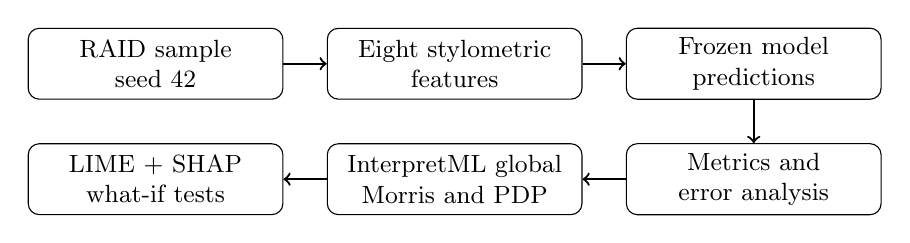
\begin{tikzpicture}[node distance=0.55cm, every node/.style={draw,rounded corners,align=center,text width=3.0cm,minimum height=0.9cm,font=\small},arr/.style={->,thick}]
\node (a) {RAID sample\\seed 42};\node[right=of a] (b) {Eight stylometric\\features};\node[right=of b] (c) {Frozen model\\predictions};\node[below=of c] (d) {Metrics and\\error analysis};\node[left=of d] (e) {InterpretML global\\Morris and PDP};\node[left=of e] (f) {LIME + SHAP\\what-if tests};
\draw[arr](a)--(b);\draw[arr](b)--(c);\draw[arr](c)--(d);\draw[arr](d)--(e);\draw[arr](e)--(f);\end{tikzpicture}\caption{Evaluation and explanation workflow}\end{figure}

\sect{4.2 Data and sample selection}
The dataset is RAID, repository \texttt{liamdugan/raid}, split \texttt{raid/train}, revision:\\
\texttt{865cac74188466cb0c3b7574a10204007b57a459}. A streaming scan found 160,452 eligible human and 5,455,368 eligible AI records. Eligible rows have English genre, nonempty generation text, and a human or AI model label. Seeded reservoir sampling (Algorithm R, seed 42) selected 5,000 from each class, with zero recorded exclusions. This is balanced by design and therefore does not represent natural prevalence. Dataset-source overlap with the detector's training data cannot be ruled out completely.

\sect{4.3 Frozen detector and feature representation}
The model is \texttt{dinisds/stylometric-ai-detector}. Its pinned revision is:\\
\texttt{de4e8a8099533b6af8a46f004d5966a7594b14a6}.\\
The artifact file is:\\
\texttt{random\_forest\_stylometric\_model.joblib} (418,937,049 bytes).
\begin{quote}\small\textbf{SHA-256 checksum:}\\
\texttt{386cfbd171eeae2f8}\\
\texttt{6a46f004d5966a7594b14a6}\\
\texttt{f32d59cdd9daa18b7144179a5347b57c}
\end{quote}
It is a 100-tree Random Forest; class 0 is Human and class 1 is AI. The project does not fit a replacement model. Since Joblib uses pickle-based deserialization, loading requires explicit \texttt{ALLOW\_PICKLE\_MODEL=1} after the pinned artifact has been reviewed.

Features, in model input order, are: (1) \texttt{char\_count}, Python Unicode code-point length; (2) \texttt{word\_count}, number of whitespace-separated tokens; (3) \texttt{avg\_word\_len}, mean token length; (4) \texttt{punct\_count}, ASCII punctuation characters; (5) \texttt{sentence\_count}, number of non-empty chunks split by one or more \texttt{. ! ?}, with minimum one; (6) \texttt{avg\_sentence\_len}, words divided by sentence count; (7) \texttt{upper\_case\_count}, alphabetic whitespace tokens satisfying \texttt{isupper}; and (8) \texttt{title\_case\_count}, tokens satisfying \texttt{istitle}. Interpretability operates on these numeric features, not raw text spans.

\sect{4.4 Explanation protocol}
The global explanation set contains 500 examples sampled from the 10,000 evaluation rows using seed 42 (256 human and 244 AI). Morris analysis uses 200 trajectories, four levels, and seed 42. Partial dependence uses ten grid points. Both methods treat numeric inputs as continuous. For local methods, a 50-row reference sample (27 human, 23 AI) is drawn with seed 42. LIME uses 3,000 perturbation samples; Kernel SHAP uses 256 samples. Four cases are chosen, one for each actual/predicted outcome category. A 12-row compatibility gate confirms adapter probabilities match the original model. A repeated-explanation stability check reports top-three Jaccard overlap. What-if analysis changes one input at a time to the evaluation sample's 10th, 50th, and 90th percentiles, leaving the other seven fixed.

\sect{4.5 Assumptions and design choices}
Balanced evaluation gives equal class weight for comparison but changes precision relative to deployment prevalence. Global results depend on the sampled 500 cases. Local attributions depend on the selected background and perturbations. Numeric feature interventions may be mutually inconsistent and may not correspond to any real text. These are model-behavior summaries, not causal interventions or proof of data-generating mechanisms.

\chap{ch:implementation}{CHAPTER 5: IMPLEMENTATION}
\sect{5.1 Environment and components}
The completed cloud execution used Python 3.12.3, InterpretML 0.6.10, and scikit-learn 1.6.1 on CPU. The source repository separates dataset loading, feature extraction, model loading, evaluation, explanation generation, and what-if analysis into modules under \texttt{src/}. Experiment settings are recorded in \texttt{configs/experiment.yaml}; the end-to-end workflow is in \texttt{notebooks/interpretml\_ai\_text\_detector.ipynb}. The model and full multi-gigabyte dataset are runtime downloads and are not committed.

\sect{5.2 Execution sequence}
The notebook installs the declared dependencies, pins and streams the dataset revision, records eligible counts and IDs, samples both labels deterministically, loads the checksum-checked model, computes predictions and metrics, runs the compatibility gate, generates global and local explanations, exports figures and structured results, then writes reports. The feature extractor is aligned with the released feature definitions. InterpretML receives a probability-predicting interface that delegates to the frozen estimator; no fit call is made on the detector.

\sect{5.3 Repository and reproducibility}
The Git repository is the \href{https://github.com/gnanendranaidun/interpretml-ai-text-detector}{GitHub project page}. Source revisions and seed are explicit. The sampled text cache and 419 MB model are excluded from Git, while sample identifiers, configurations, code, figures, and reports are versioned. Reproduction requires access to the pinned public model and dataset revisions and sufficient storage/time to stream the RAID training split.

\chap{ch:results}{CHAPTER 6: RESULTS AND DISCUSSION}
\sect{6.1 Classification performance}
\begin{table}[H]\centering\caption{Performance on the balanced 10,000-record sample}\begin{tabular}{lr}\hline Measure & Result\\\hline Accuracy & 0.6099\\AI precision & 0.5966\\AI recall & 0.6790\\AI F1 & 0.6351\\AI ROC-AUC & 0.6445\\\hline\end{tabular}\end{table}
The confusion matrix is \([ [2704,2296], [1605,3395] ]\), with rows as actual Human/AI and columns as predicted Human/AI. The detector correctly classified 2,704 of 5,000 human examples and 3,395 of 5,000 AI examples. It produced 2,296 human-to-AI errors and 1,605 AI-to-human errors. The model card's 96.03\% is an author-reported result on a different evaluation and was not reproduced here.
\begin{figure}[H]\centering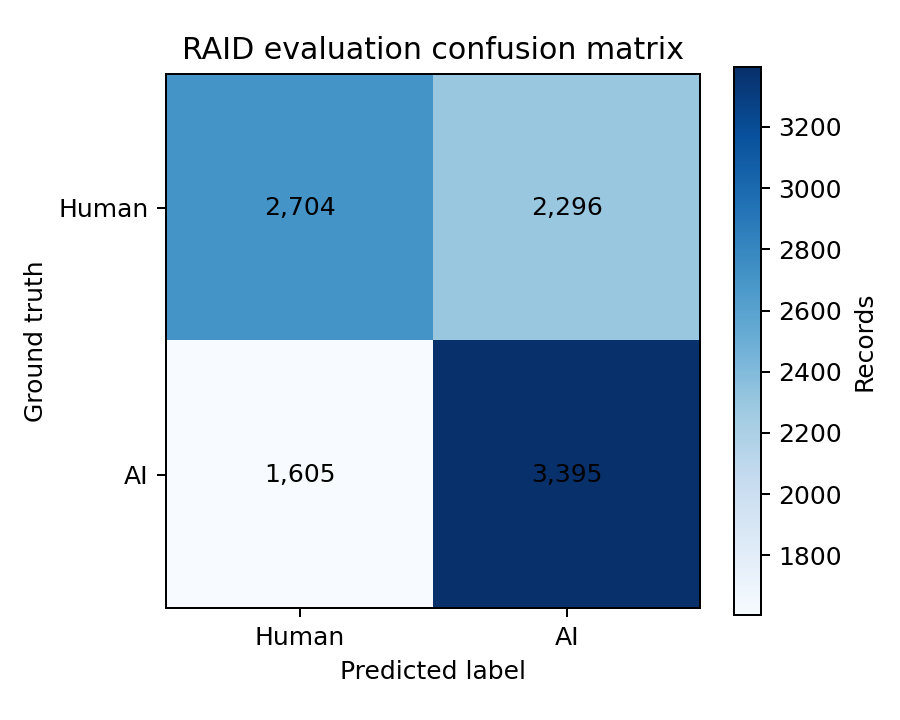
\includegraphics[width=0.58\textwidth]{images/confusion_matrix.png}\caption{Confusion matrix for the balanced evaluation sample}\end{figure}

\sect{6.2 Global feature behavior}
Morris mean absolute elementary effects ranked average word length highest (0.3276), followed by word count (0.13395), character count (0.103275), punctuation count (0.097875), title-case count (0.077775), sentence count (0.071625), uppercase count (0.0468), and average sentence length (0.042825). The reported convergence index is 0.2243835. These are screening scores over the selected feature region and scales; they do not indicate causal importance or comparable real-world effect units.
\begin{figure}[H]\centering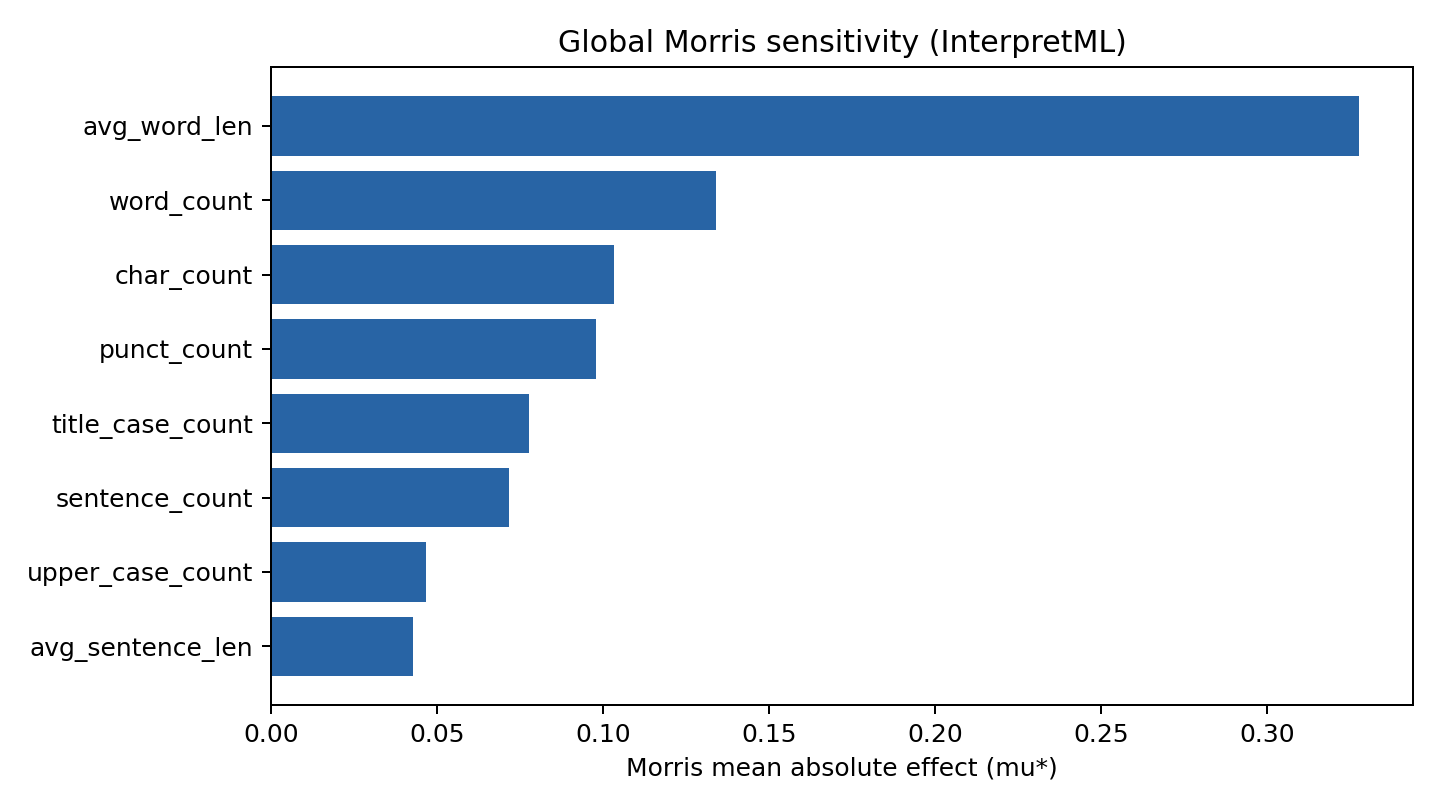
\includegraphics[width=0.88\textwidth]{images/morris_sensitivity.png}\caption{Morris global sensitivity results}\end{figure}

Partial dependence illustrates average probability response over the selected sample. The first-to-last grid P(AI) values include average word length 0.303 to 0.881, word count 0.671 to 0.336, character count 0.573 to 0.429, and punctuation count 0.474 to 0.658. Curves can be non-monotonic and should not be read as interventions on actual prose. For correlated or impossible combinations, partial dependence may average over feature vectors that do not occur naturally.
\begin{figure}[H]\centering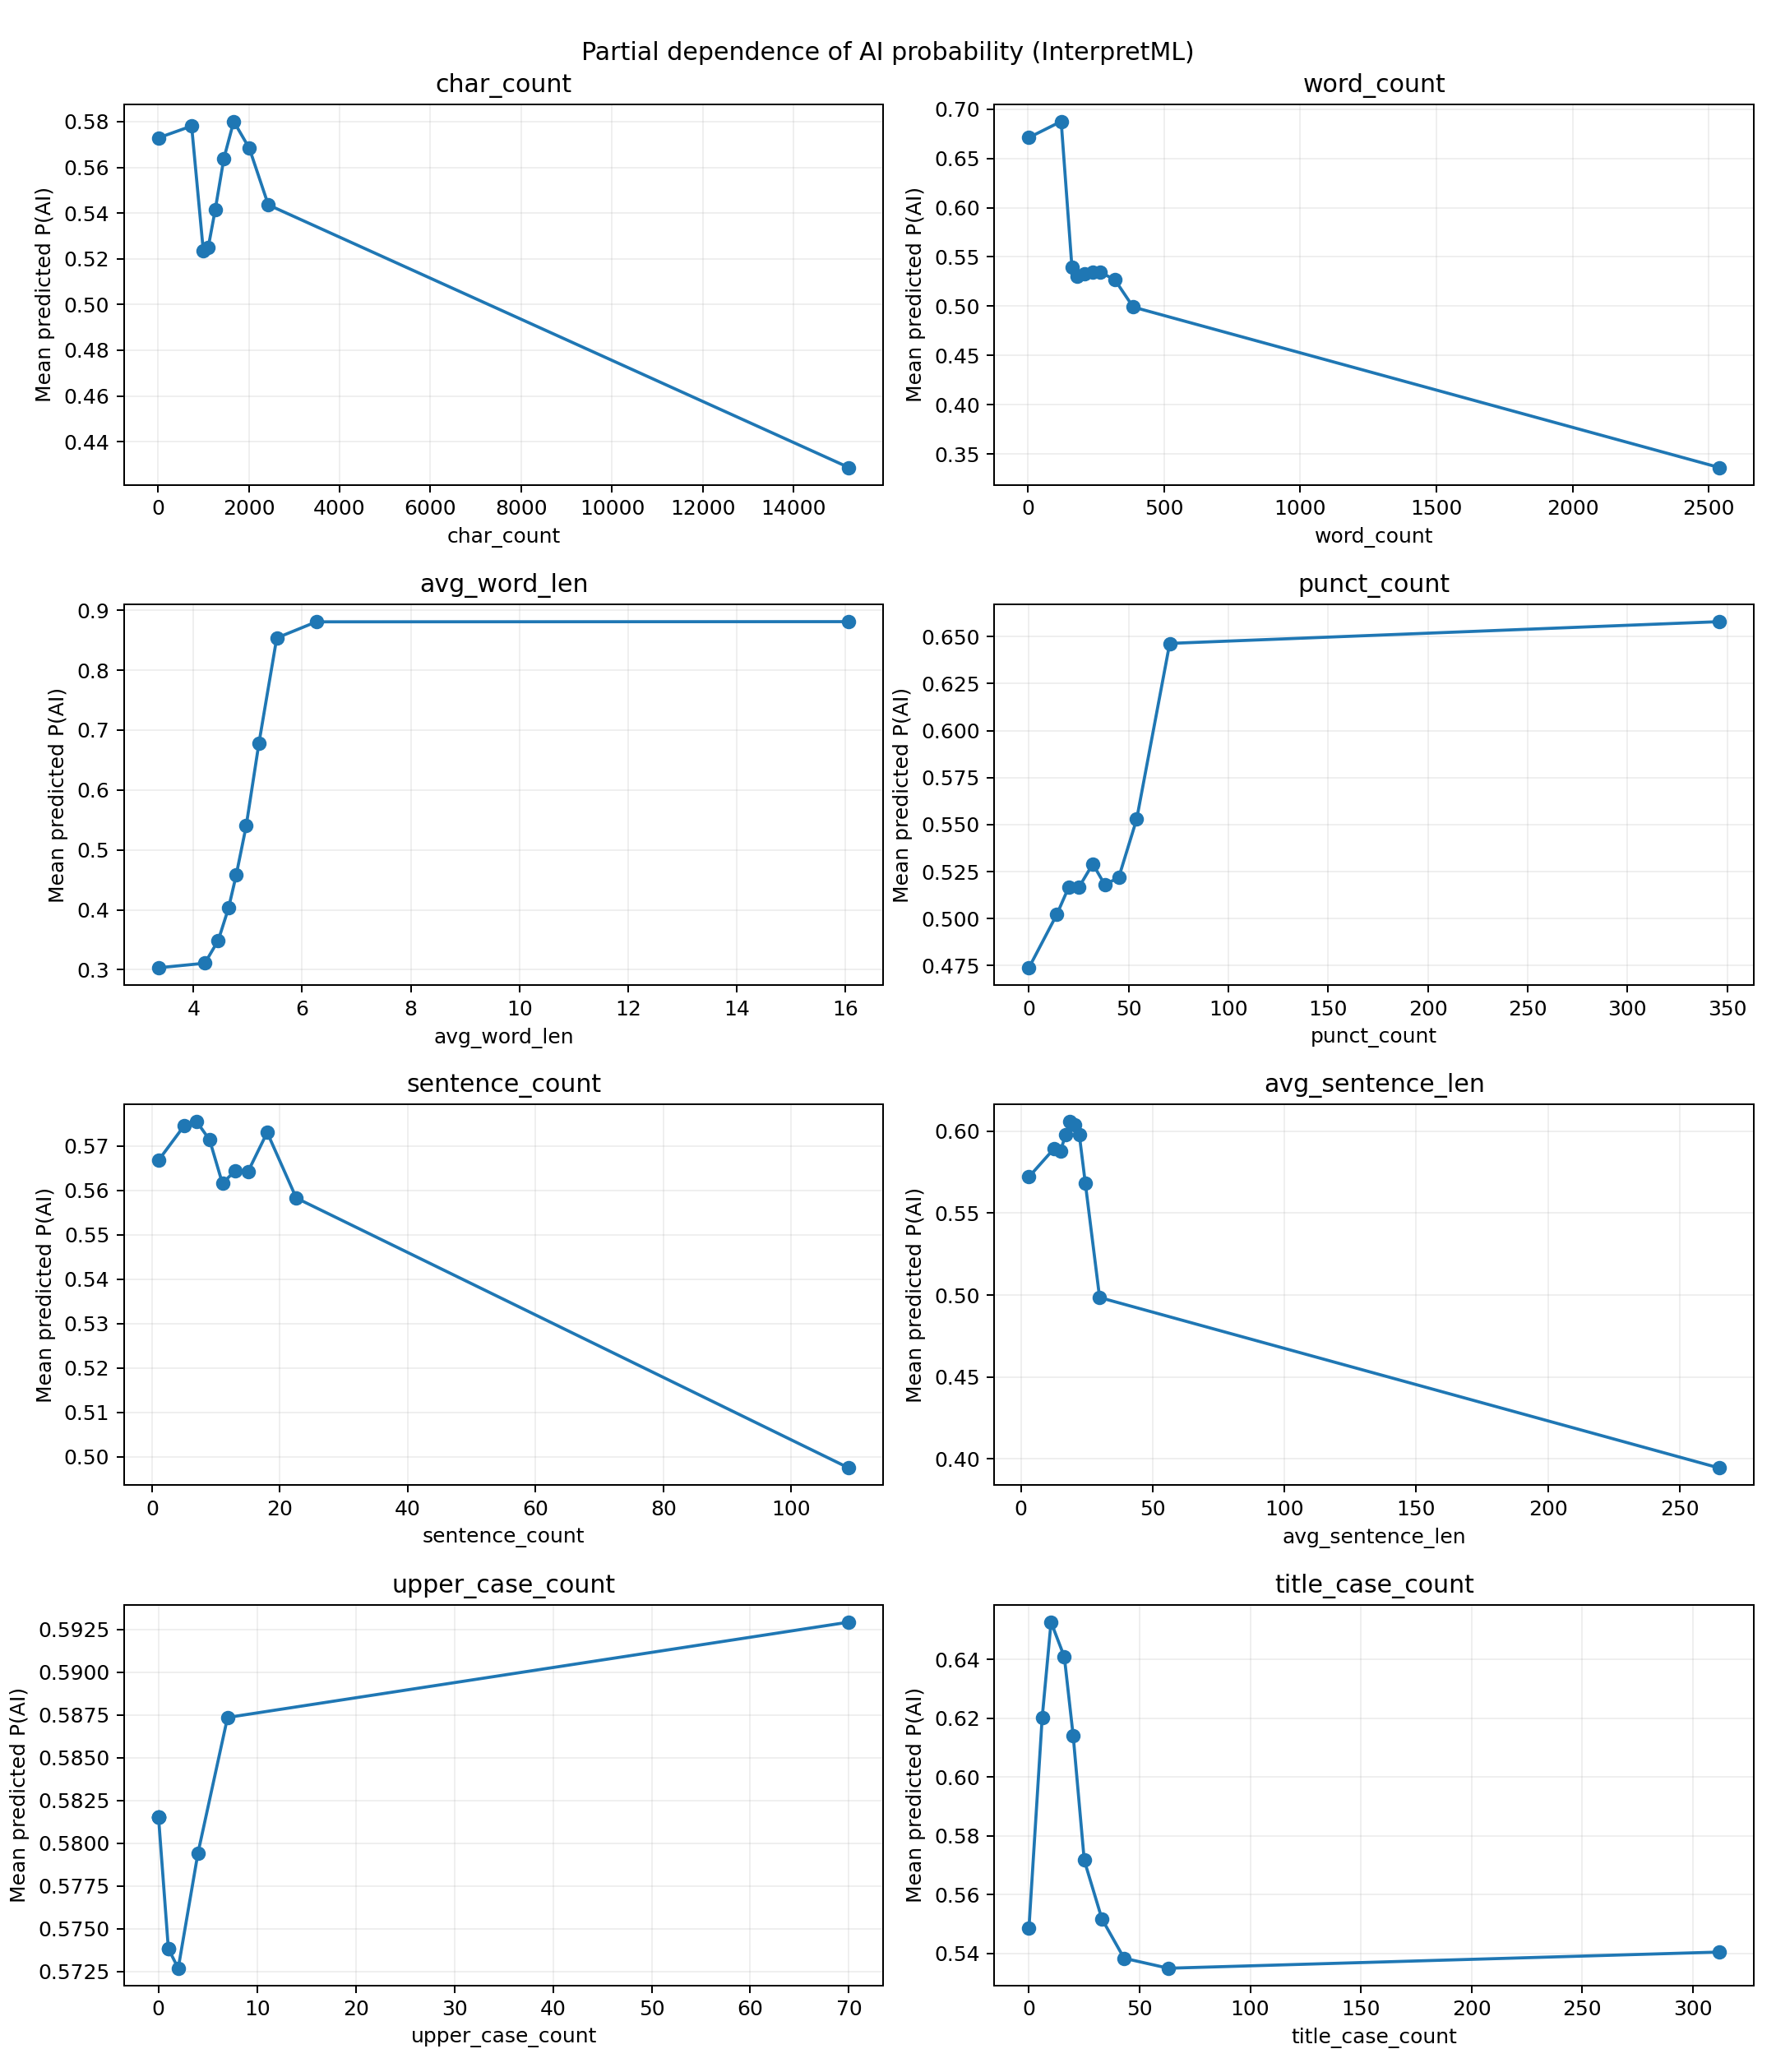
\includegraphics[width=0.9\textwidth]{images/partial_dependence.png}\caption{Partial dependence across eight numeric inputs}\end{figure}

\sect{6.3 Local cases}
\begin{table}[H]\centering\caption{Representative local outcomes}\small\begin{tabularx}{\textwidth}{l l l X}\hline Case & Actual/predicted & P(Human), P(AI) & Leading local signal\\\hline Correct AI & AI / AI & 0.10, 0.90 & Average word length supports AI; average sentence length offsets it\\Correct human & Human / Human & 0.59, 0.41 & Contributions are small and method-dependent\\Human labeled AI & Human / AI & 0.38, 0.62 & Punctuation and average word length are prominent\\AI labeled human & AI / Human & 1.00, 0.00 & Average word and sentence length support Human\\\hline\end{tabularx}\end{table}
LIME and Kernel SHAP both identified average word length as the largest positive AI contribution for the correctly classified AI case. In the human-mislabeled-as-AI case, local ranking differed across methods: punctuation was prominent for LIME, while average word length was prominent for SHAP. In the AI-mislabeled-as-human case, both methods associated shorter average word length with the Human output. Agreement or disagreement is about approximate model behavior in the chosen neighborhood; it does not validate the prediction. Top-three Jaccard overlap under the configured repeat check was 1.0 for both methods across all four cases.

\sect{6.4 What-if analysis}
The 96 perturbations (four cases, eight features, three quantiles) generated 14 prediction flips. The largest observed probability change was for the correctly detected AI example when average word length was changed to its 10th-percentile value: P(AI) moved from 0.90 to 0.07. The correctly classified human case flipped in five perturbations, the human mislabeled as AI in six, the AI mislabeled as human in one, and the correct AI case in two. The result demonstrates local numerical sensitivity; constructed feature combinations may not represent valid text and should not be interpreted as actionable editing advice.

\sect{6.5 Objective achievement and validity limits}
All implementation objectives were achieved: pinned frozen inference, balanced evaluation, metrics, compatibility check, global and local interpretation, what-if analysis, and versioned outputs. The run establishes performance only for this artifact and sample protocol. Limitations include the pooled English data, balanced class prior, possible train-source overlap, model age, feature engineering's narrow surface view, no threshold calibration, and no evaluation across people, genres, attacks, or languages. Explanations are sample- and method-dependent. The observed results do not support using the detector for disciplinary or individual authorship decisions.

\chap{ch:conclusion}{CHAPTER 7: CONCLUSION}
This project completed a reproducible evaluation and interpretation workflow for a frozen stylometric AI-text detector. On 10,000 balanced RAID records it reached 60.99\% accuracy and 0.6445 AI ROC-AUC, with thousands of errors in both directions. InterpretML methods exposed which numeric features influenced the fixed model globally and in selected local cases. Average word length ranked highest in global Morris sensitivity, while local explanations and counterfactual-like perturbations showed case-specific behavior. Results reinforce that detector outputs depend on a narrow feature representation and evaluation distribution. The main outcome is an auditable description of this detector's behavior, not a validated authorship test.

\chap{ch:future}{CHAPTER 8: FUTURE WORK}
Future work can evaluate unbalanced and prevalence-sensitive settings, report precision-recall curves and calibrated operating thresholds, stratify by RAID domain, generator, decoding, and attack, and conduct a separate multilingual and non-native-writer fairness audit. Robustness testing should include paraphrase and formatting transformations. Feature-level explanations can be compared with controlled synthetic texts to test whether sensitivities persist under coherent edits. A future study could compare additional frozen detectors under a preregistered protocol, audit source overlap more deeply, and assess explanation stability under alternative backgrounds. Any threshold or use recommendation would need validation for its specific context and should not convert a probabilistic score into an authorship verdict.

\clearpage\begin{center}{\bfseries\fontsize{16}{20}\selectfont REFERENCES}\end{center}
{\small\sloppy\begin{enumerate}[leftmargin=*,itemsep=1pt]
\item Gehrmann, S., Strobelt, H., and Rush, A. M. (2019). GLTR: Statistical Detection and Visualization of Generated Text. ACL System Demonstrations, 111--116. \href{https://aclanthology.org/P19-3019/}{source}
\item Uchendu, A., Ma, Z., Le, T., Zhang, R., and Lee, D. (2021). TURINGBENCH: A Benchmark Environment for Turing Test in the Age of Neural Text Generation. Findings of EMNLP, 2001--2016. \href{https://aclanthology.org/2021.findings-emnlp.172/}{source}
\item Rodriguez, J. D., Hay, J., Gros, D., Shamsi, J. A., and Srinivasan, P. (2022). Cross-Domain Detection of GPT-2-Generated Technical Text. NAACL-HLT, 1213--1233. \href{https://aclanthology.org/2022.naacl-main.88/}{source}
\item Liang, W., Yuksekgonul, M., Mao, Y., Wu, E., and Zou, J. (2023). GPT detectors are biased against non-native English writers. Patterns, 4(7), 100779. \\\href{https://doi.org/10.1016/j.patter.2023.100779}{DOI}.
\item Mitchell, E., Lee, Y., Khazatsky, A., Manning, C. D., and Finn, C. (2023). DetectGPT: Zero-Shot Machine-Generated Text Detection using Probability Curvature. ICML, PMLR 202, 24950--24962. \href{https://proceedings.mlr.press/v202/mitchell23a.html}{source}
\item Yang, X. et al. (2024). DNA-GPT: Divergent N-Gram Analysis for Training-Free Detection of GPT-Generated Text. ICLR. \href{https://arxiv.org/abs/2305.17359}{source}
\item Macko, D. et al. (2023). MULTITuDE: Large-Scale Multilingual Machine-Generated Text Detection Benchmark. EMNLP, 9960--9987. \href{https://aclanthology.org/2023.emnlp-main.616/}{source}
\item Wang, Y. et al. (2024). M4: Multi-generator, Multi-domain, and Multi-lingual Black-Box Machine-Generated Text Detection. EACL, 1369--1407. \href{https://aclanthology.org/2024.eacl-long.83/}{source}
\item Li, Y. et al. (2024). MAGE: Machine-generated Text Detection in the Wild. ACL, 36--53. \href{https://aclanthology.org/2024.acl-long.3/}{source}
\item Bao, G. et al. (2024). Fast-DetectGPT: Efficient Zero-Shot Detection of Machine-Generated Text via Conditional Probability Curvature. ICLR. \href{https://proceedings.iclr.cc/paper_files/paper/2024/file/6b8c6f846c3575e1d1ad496abea28826-Abstract-Conference.html}{source}
\item Verma, V., Fleisig, E., Tomlin, N., and Klein, D. (2024). Ghostbuster: Detecting Text Ghostwritten by Large Language Models. NAACL-HLT, 1702--1717. \href{https://aclanthology.org/2024.naacl-long.95/}{source}
\item Hans, A. et al. (2024). Spotting LLMs With Binoculars: Zero-Shot Detection of Machine-Generated Text. ICML, PMLR 235, 17519--17537. \href{https://proceedings.mlr.press/v235/hans24a.html}{source}
\item Dugan, L. et al. (2024). RAID: A Shared Benchmark for Robust Evaluation of Machine-Generated Text Detectors. ACL, 12463--12492. \href{https://aclanthology.org/2024.acl-long.674/}{source}
\item Wang, Y. et al. (2024). Stumbling Blocks: Stress Testing the Robustness of Machine-Generated Text Detectors Under Attacks. ACL, 2894--2925. \href{https://aclanthology.org/2024.acl-long.160/}{source}
\item Sadasivan, V. S. et al. (2025). Can AI-Generated Text Be Reliably Detected? Stress Testing AI Text Detectors Under Various Attacks. TMLR. \href{https://openreview.net/pdf?id=OOgsAZdFOt}{source}
\item Tufts, B., Zhao, A., and Li, S. (2025). A Practical Examination of AI-Generated Text Detectors for Large Language Models. Findings of NAACL, 4839--4856. \href{https://aclanthology.org/2025.findings-naacl.271/}{source}
\item Doughman, J. et al. (2025). Exploring the Limitations of Detecting Machine-Generated Text. COLING, 4274--4281. \href{https://aclanthology.org/2025.coling-main.288/}{source}
\item Dutta Chowdhury, S. A., Espana-Bonet, C., and Van Genabith, J. (2026). Formatting and Surface Feature Confounds in AI Text Detection: A Clever Hans Effect. Findings of EMNLP, 22266--22277. \href{https://aclanthology.org/2026.findings-emnlp.1051/}{source}
\item El Attar, A., Donmez, C., Maurer, M., and Falenska, A. (2026). A Systematic Analysis of Linguistic Features in AI-Generated English Text Detection Across Domains and Models. Findings of IJCNLP-AACL, 181--208. \href{https://aclanthology.org/2026.findings-aacl.10/}{source}
\item Xia, M., Stanczak, K., and Roth, B. (2026). Explaining Generalization of AI-Generated Text Detectors Through Linguistic Analysis. EACL, 6524--6546. \href{https://aclanthology.org/2026.eacl-long.307/}{source}
\item Ribeiro, M. T., Singh, S., and Guestrin, C. (2016). Why Should I Trust You? Explaining the Predictions of Any Classifier. KDD, 1135--1144. \\\href{https://doi.org/10.1145/2939672.2939778}{DOI}.
\item Lundberg, S. M. and Lee, S.-I. (2017). A Unified Approach to Interpreting Model Predictions. NeurIPS. \href{https://proceedings.neurips.cc/paper/2017/hash/8a20a8621978632d76c43dfd28b67767-Abstract.html}{source}
\item Morris, M. D. (1991). Factorial Sampling Plans for Preliminary Computational Experiments. Technometrics, 33(2), 161--174. \\\href{https://doi.org/10.1080/00401706.1991.10484804}{DOI}.
\item Friedman, J. H. (2001). Greedy Function Approximation: A Gradient Boosting Machine. The Annals of Statistics, 29(5), 1189--1232. \\\href{https://doi.org/10.1214/aos/1013203451}{DOI}.
\item Nori, H., Jenkins, S., Koch, P., and Caruana, R. (2019). InterpretML: A Unified Framework for Machine Learning Interpretability. arXiv:1909.09223. \href{https://arxiv.org/abs/1909.09223}{source}
\end{enumerate}}
\clearpage\chap{app:appendix}{APPENDIX: REPRODUCTION NOTES}
The repository README gives environment setup. In summary: clone the GitHub repository, install \texttt{requirements.txt}, open the experiment notebook, and run cells in order. Before loading the pinned Joblib artifact, review its revision and SHA-256 in \texttt{models/README.md}, then set \texttt{ALLOW\_PICKLE\_MODEL=1}. Dataset scanning transfers and processes a large training split and can take substantial time. No GPU is required. Generated deliverables are included with this report; full source data and model binaries are not redistributed in the repository.

\end{document}
